\section{Introduction}

Improving user retention and preventing user churn have become an important focus for many internet companies as the market matures and the cost of acquiring new users rises. In addition to the natural friction, experiencing bad service is one of the main driving factors behind user churn. In different industries, companies provide different services; examples include accommodation (Airbnb), ride-sharing (Uber, Lyft), and e-commerce (Amazon, Ebay).

As suggested in a previous research study from Uber \cite{halperin2018toward}, providing a user with a promotion without explicit apology after a dissatisfied trip experience (for instance, unreliable arrival times) will have a positive treatment effect on future billings. This is also consistent with the finding in another study \cite{cohen2018frustration} where researchers conducted a similar experiment on Via (a ride-sharing company in NYC). However, as a common practice, these previous research studies rely solely on non-causal churn prediction or heuristics based on frustrating experiences for promo decisions instead of directly optimizing the promotional heterogeneous treatment effect.

The goal of our work is to maximize the treatment effect of promotions on user retention in order to reduce user churn (especially caused by experiencing an unsatisfactory service) under a cost constraint. Compared to existing work on user promotions and heterogeneous treatment effect estimation, novel contributions of this paper are:
\begin{itemize}
\item \textbf{Treatment Effect based Promo Decision} 

A common approach for promotion decision relies on regular predictions, redemption, or heuristics which are tied to specific scenarios and require rich background context. In this paper, we propose a general framework that directly optimizes the promotional heterogeneous treatment effect and could be applied to various business use cases with minimum change.

\item \textbf{Heterogeneous Treatment Efficiency Optimization} 

Most of the research studies focus on the treatment effect of one single value and treat the cost of that treatment as fixed. However, in many cases it is also necessary to estimate the treatment effect on the cost and use the efficiency ratio of $\Delta$value/$\Delta$cost when making the resource allocation decision. Two algorithms we propose will address this case.

\item \textbf{Ranking for Aggregated Treatment Effect} 

Similar to the case of search ranking vs point estimate of Click Through Rate (CTR), here our objective is to maximize aggregated treatment effect instead of having a perfect point estimate of individual treatment effect and thus we could achieve better performance by moving from point estimate to ranking. We propose a novel algorithm to solve this treatment effect ranking problem.

\item \textbf{Empirical Evaluation Method} 

A common difficulty in comparing the accuracy of heterogeneous treatment effect estimators on real data is that we do not have access to the ground truth. The alternative adopted by some research is the uplift curve \cite{rzepakowski2012decision}. In this paper we propose the "cost curve", a metric designed for the efficiency ratio case above that is consistent with live performance.

\end{itemize}
The structure of this paper is as follows: in section 2, we will cover some preliminaries for heterogeneous treatment effects and the importance of considering treatment effect on cost instead of treating it as a fixed factor. In section 3, we will talk about evaluation metrics (e.g. cost curve) and our modeling approaches for heterogeneous treatment effect optimization. In section 4, we will cover experiment design for data collection, model offline comparison and real-world performance from the product we already launched. Finally, we would briefly cover the related work and future research steps.

\section{Preliminaries}

\subsection{Heterogeneous Treatment Effect}

We formalize our problem in terms of the potential outcomes framework \cite{rubin1974estimating}. We have $n$ independent and identically distributed examples $(X_i, Y_i, W_i), i = 1, ..., n$, where $X_i \in \chi$ denotes per-sample features, $Y_i \in \mathbb{R}$ is the observed outcome, and $W_i \in \{0, 1\}$ is the treatment assignment. We posit the existence of potential outcomes $\{Y_i(0), Y_i(1)\}$ corresponding to the outcome we would have observed given the treatment assignment $W_i = 0$ or $1$ respectively, such that $Y_i = Y_i(W_i)$ and try to estimate the conditional average treatment effect (CATE) function 
\begin{equation}
  \label{eq:1}
  \tau(x) = \mathbb{E}[Y(1)-Y(0) | X = x]
\end{equation}
We assume unconfoundedness, i.e., the treatment assignment is as good as random once we control for the features $X_i$ \cite{rosenbaum1983central}.
\begin{equation}
  \label{eq:2}
  \{Y_i(0), Y_i(1)\} \perp W_i|X_i
\end{equation}
We write the treatment propensity as $e(x) = \mathbb{P} [W = 1  | X = x]$.

In our case we have fully controlled randomized experiment, which means we have a stronger assumption than unconfoundedness:
\begin{equation}
  \label{eq:3}
  \{Y_i(0), Y_i(1)\} \perp W_i
\end{equation}
And therefore, we have $e(x) = p$ while $p$ is the overall treatment percentage. We also have the specific meaning for each variable mentioned above as follow:
\begin{itemize}
\item $X$: per trip features
\item $Y^r$: binary user retention outcome in a given period, 1 means this user took at least 1 trip and 0 means churn
\item $Y^c$: net cost of this user in a given period, which is the sum of net cost of each trip this user has taken
\item $\tau^r$: user level promotional treatment effect on retention
\item $\tau^c$: user level promotional treatment effect on net cost
\end{itemize}

\subsection{Problem Statement}
We want to maximize the aggregated promotional treatment effect on user retention given a promotion cost constraint. This requires us to identify a subgroup of samples that is more efficient and thus provide a higher aggregated treatment effect. This could be described in Eq. (\ref{eq:problem_statement}) where $z_i$ is the binary variable indicates whether we select that sample into our subgroup and $B$ is the promotion cost budget.
\begin{equation}
  \label{eq:problem_statement}
  max \sum_{i=1}^n\tau^r(x_i)z_i \quad 
  s.t. \sum_{i=1}^n\tau^c(x_i)z_i \leq B, \ z_i \in \{0, 1\}
\end{equation}

Note here we won't have selection bias for heterogeneous treatment effect estimation regarding decision variable $z_i$ as our treatment control split is after $z_i$ has been determined. This means $z_i \perp W_i$.

\subsection{Treatment Effect on Cost over Fixed Cost}
Most research studies treat the cost of applying the treatment as fixed. Taking promotion for example, they would use the fixed coupon value as the promo cost. However, this does not accurately account for the incremental profit generated by behavior change induced by the promotion.

Two users might have the same incremental retention effect but one could have a higher usage and thus contribute a larger incremental profit. This can only be captured by measuring the treatment effect on net cost.

\section{Model}

In this section, we will cover an evaluation metric closely related to our business use case and introduce various models to solve the optimization problem mentioned above.

\subsection{Model Evaluation Metric}
The business objective is to achieve most incremental user retention with a given promotion cost budget. The retention and cost here are 2 critical values mentioned above for the causal ratio. 

\textbf{Cost curve.} Now that we have 2 treatment outcomes $\tau^r$ and $\tau^c$ we care about, we draw a curve and use incremental cost as X-axis and incremental value (retention in this case) as Y-axis as illustrated in Figure \ref{fig:cost_curve_illustration}. 
\begin{figure}
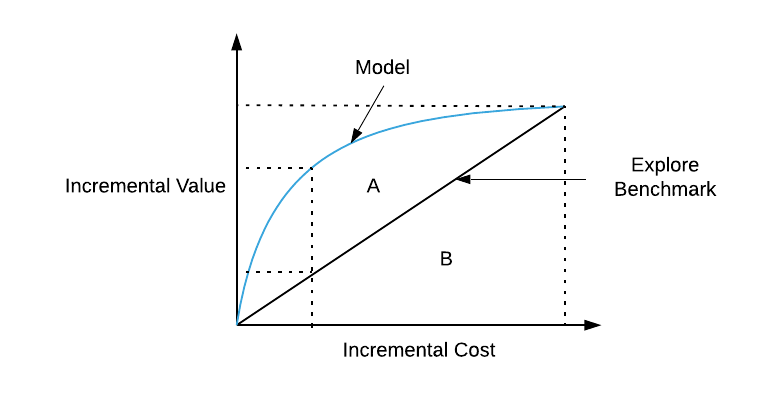
\includegraphics[height=2in]{cost_curve_illutration}
\Description{Cost curve illustration}
\caption{Illustration for cost curve, X and Y axis are treatment effect on cost and value respectively. Moving along the curve from origin to top right, we gradually increase the sample included based on ranking score.}
\label{fig:cost_curve_illustration}
\end{figure}
Similar to uplift curve \cite{rzepakowski2012decision}, assume we have a score for each sample $S_i=f(X_i)$ that represents how good the sample is regarding the incremental cost and value. We could order samples by this score, then each point on the curve could be calculated from the $p$ percent highest scored samples. The value for X and Y axis for each point could be calculated respectively by Eq. (\ref{eq:point_on_cc}), taking the number of treatment samples times ATE (Average Treatment Effect) of this group.
\begin{equation}
  \label{eq:point_on_cc}
  \#\{W_i=1|S_i>S^{p_{th}}_i\} \times ATE\{x_i|S_i>S^{p_{th}}_i\}
\end{equation}
Note we can score the samples for both treatment and control as $f$ does not depend on $W$. Here function $f$ is the one we want to learn and we will discuss it in more details in the following section.

Figure \ref{fig:cost_curve_illustration} represents the idea of the cost curve: as you increase the percent $p$ of samples to be included for each point, the aggregated incremental cost and value would increase (since you include more samples). So the end point of the cost curve (top right) is the one that includes all samples. And the origin (down left) is the one includes no sample.

If the score $S_i$ is randomly generated, then there would be no difference between high and low score points regarding the ratio of incremental cost and value, and thus the cost curve should be a straight line. However, if the score is generated by a good model, then the curve should be above the benchmark line. This means for the same level of incremental cost, a better model would select samples to achieve higher incremental value.

\textbf{Area Under Cost Curve (AUCC).} Similar to Area Under Uplift Curve and AUC of ROC curve, here we use the area under cost curve as the numerical metric. To normalize the value, we use the ratio $A/B$ as the AUCC, where $A$ is the area between model curve and the benchmark curve, and $B$ is the area under benchmark curve (shown in Figure \ref{fig:cost_curve_illustration}). The equivalent formula for AUC of ROC curve is $(A+B)/2B = A/2B + 0.5$ where $A/B$ is the value that matters. The theoretical upper bound of $A$ is $B$ (the symmetric upper triangle), which means with no incremental cost we can achieve all incremental value from the sample. So this $A/B$ should be bounded within $[0, 1)$ and larger the AUCC, generally better the model. One might argue that the model curve could below the benchmark line if the model is really bad, and thus $A$ could be negative. However if that's the case, we can always achieve a positive $A$ by reversing the ranking score from this bad model. So the worst we can achieve is the random explore benchmark line.

\subsection{Cardinal Prediction}
Most of the existing estimators provide cardinal prediction for one single outcome metric and we need to adjust it to account for treatment effect ratio between value and cost for our case. In this section we describe how we adjust existing estimators with Lagrangian Subgradient method to maximize the total treatment effect on user retention with a given promotion cost budget.

Here we consider R-learner \cite{nie2017quasi} and Causal Forest \cite{wager2017estimation} as the treatment effect estimators. R-learner is a synthetic control fashion two-step algorithm that estimates the marginal effect and then isolates the causal component. Causal Forest is a matching fashion tree-based ensemble algorithm that partitions both treatment and control samples based on their features and directly estimates the treatment effect under each tree leaf. Generally, we can train above models and have cardinal predictions $\hat\tau(x_i)$ for value (retention) and cost. 

\textbf{Individual Causal Ratio.} Given cardinal prediction $\hat\tau(x_i)$ for value and cost, our problem is actually a 0-1 knapsack problem:
\begin{equation}
  \label{eq:knapsack}
  max \sum_{i=1}^n\hat\tau^r(x_i)z_i \quad 
  s.t. \sum_{i=1}^n\hat\tau^c(x_i)z_i \leq B, \ z_i \in \{0, 1\}
\end{equation}
where $z_i$ is the binary indicator of promo decision and $B$ is the promo cost budget. It's not feasible to directly solve this knapsack problem due to the large number of items. Because the $\tau^c$ of each item is much smaller than the total budget and we can always deviate a certain amount from the budget, the capacity constraint can be relaxed and this problem can be well approximated by a fractional knapsack problem \cite{dantzig1957discrete} and the greedy algorithm of selecting items with smallest $\tau^c/\tau^r$ can be good enough and efficient. To get the ratio, we need to train 2 models, one for $\hat{\tau}^c$ and the other for $\hat{\tau}^r$, then we use Eq.(\ref{eq:causal_ratio})
\begin{equation}
  \label{eq:causal_ratio}
  S_i=\frac{\hat{\tau}^r(x_i)}{\hat{\tau}^c(x_i)}
\end{equation}
as the ranking score (higher the score, better the sample).

\textbf{Lagrangian.} There are several issues with the approach above. The first is noisiness. The treatment effect prediction is extremely noisy and the ratio will amplify that. Many users will have small promotional treatment effect, which means we have a lot of zero division in this ratio. We also need to take special care with the sign of the score. For example, we want to give promo to user with $\tau^r > 0, \ \tau^c < 0$ but not vice versa. However, the ratio will not distinguish these 2 cases. Additionally, from a system perspective, we need to maintain two sets of models, one for retention and one for cost. Considering some models are two-step (like R-learner), the total number of models we need to manage becomes four, which is not ideal.

The optimization problem above actually could be rewritten in a Lagrangian form with the relaxation of binary constraint on $z_i$:
\begin{equation}
  \label{eq:lagrangian}
  max \ g=\sum_{i=1}^n\tau^r(x_i)z_i + \lambda (B-\sum_{i=1}^n\tau^c(x_i)z_i) \quad s.t. \ 0\leq z_i \leq 1
\end{equation}
We can use the subgradient method here. Starting with any initial value $\lambda$, as $\lambda$ and $\ B$ are constants, our optimization problem becomes:
\begin{equation}
  \label{eq:lagrangian_reduced}
  max \ g=\sum_{i=1}^n\tau^r(x_i)z_i - \lambda\sum_{i=1}^n\tau^c(x_i)z_i
\end{equation}
And $g$ could be rewritten as Eq. (\ref{eq:lagrangian_reduced_2}). 
\begin{equation}
  \label{eq:lagrangian_reduced_2}
  g=\sum_{i=1}^n(\tau^r(x_i)-\lambda\tau^c(x_i))z_i
\end{equation}
This optimization problem has a heuristic solution:
\begin{equation}
  \label{eq:lagrangian_heuristic_solution}
  \tau^r(x_i)-\lambda\tau^c(x_i)>0, \ z_i=1, \ o/w, \ z_i=0
\end{equation}
Plugging in this solution and taking the derivative of $g$ w.r.t $\lambda$, we have Eq. (\ref{eq:lagrangian_gradient}) where $z_i$ is the solution from Eq. (\ref{eq:lagrangian_heuristic_solution}). And we could update $\lambda$ by Eq. (\ref{eq:update_lambda}) where $\alpha$ is the learning rate.
\begin{equation}
  \label{eq:lagrangian_gradient}
  \frac{\partial g}{\partial \lambda}=B-\sum_{i=1}^n\tau^c(x_i)z_i
\end{equation}
\begin{equation}
  \label{eq:update_lambda}
  \lambda\rightarrow \lambda + \alpha(B-\sum_{i=1}^n\tau^c(x_i))
\end{equation}
Based on the heuristic solution and the gradient, we could iteratively solve for $\lambda$ \cite{bertsekas1999nonlinear} .

Now, instead of using the ratio, we could use Eq. (\ref{eq:lagrangian_score}) as our ranking score. The intuition is that the Lagrangian solution suggests we should include any sample with $\hat\tau^S(x_i)>0$. Larger this value, more contribution the sample will have and thus a higher ranking it should get.
\begin{equation}
  \label{eq:lagrangian_score}
  S_i=\hat\tau^S(x_i)=\hat\tau^r(x_i)-\lambda\hat\tau^c(x_i)
\end{equation}
This form is linear, so we have Eq. (\ref{eq:lagrangian_linearity}).
\begin{equation}
  \label{eq:lagrangian_linearity}
  \tau^r(x) - \lambda \tau^c(x) = \mathbb{E}[(Y^r(1) - \lambda Y^c(1)) - (Y^r(0) - \lambda Y^c(0)) | X = x]
\end{equation}
This means we could use $Y^S=Y^r-\lambda Y^c$ to replace the original $Y$ (single outcome for value and cost respectively) in the estimators above. Then we train a model with this $Y^S$ and the output becomes $\hat\tau^S$ which could be used directly.

The iterative process to solve $\lambda$ could be slow as the value function $g$ here is piece-wise linear w.r.t $\lambda$. We take the approach to treat $\lambda$ as a hyper-parameter and determine its value through hyper-parameter optimization. 

This Lagrangian helps us get rid of the instability of the ratio and the burden of having multiple models; and it proves to have better performance than the ratio version in both offline evaluation and online real world tests. Figure \ref{fig:cc_lagrangian_vs_ratio} shows the out-of-sample test cost curve comparison between Lagrangian and Causal Ratio using Causal Forest. We used data collected from our promotion experiment (details in \ref{experiment design and ata}) and optimize hyper-parameters with forward validation(details in \ref{offline test setup}). We can see that the Lagrangian model dominates the Causal Ratio model.
\begin{figure}
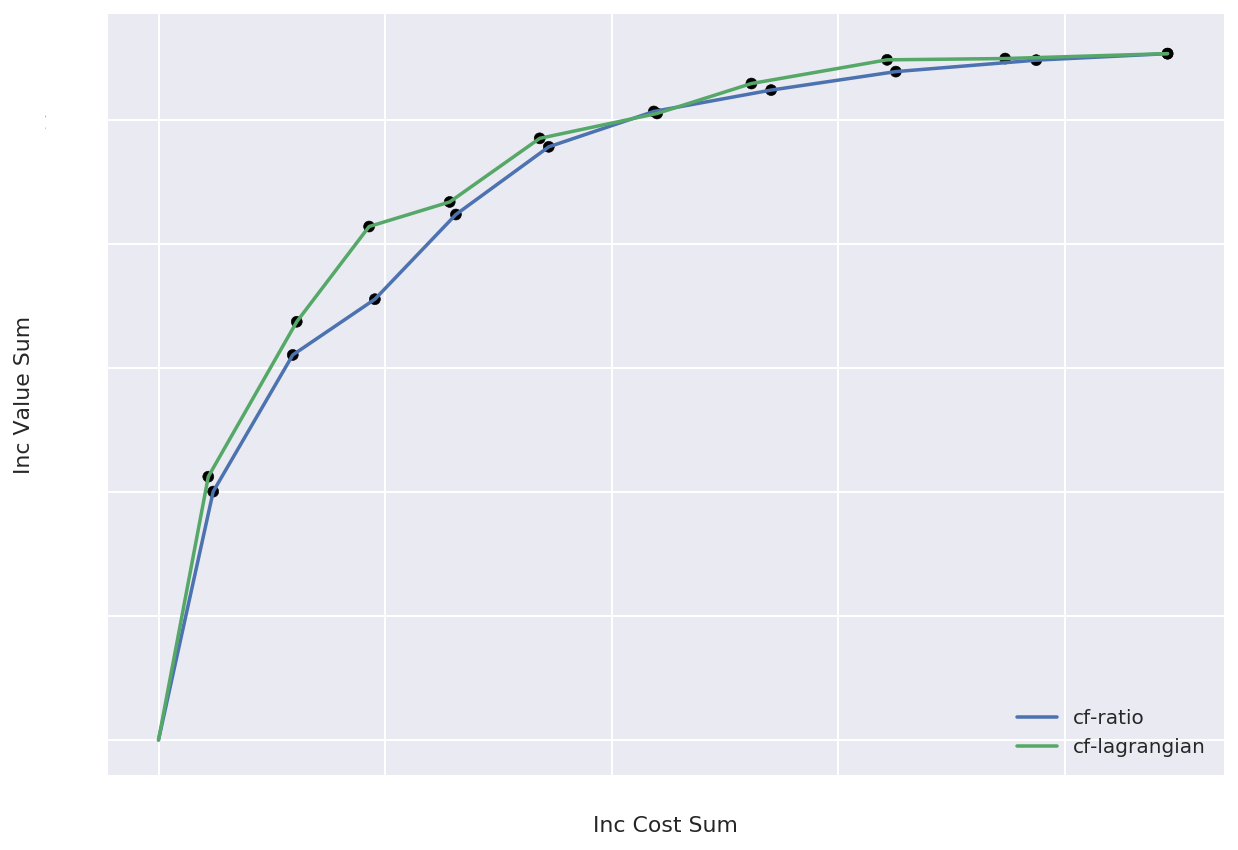
\includegraphics[height=2.2in]{cc_lagrangian_vs_ratio}
\Description{Cost Curve Lagrangian vs Ratio}
\caption{Out-of-sample cost curve comparison between Lagrangian and causal ratio using Causal Forest. Lagrangian (green curve) dominates causal ratio (blue curve).}
\label{fig:cc_lagrangian_vs_ratio}
\end{figure}

\subsection{Ordinal Prediction}
The approach described in the previous section actually contains two steps, prediction and optimization. However, the ultimate business objective is to identify a portfolio of users or trips that we can achieve highest incremental user retention with a promo cost budget, which does not rely on the perfect individual cardinal prediction (point estimate). This is similar to the search ranking algorithm vs Click Through Rate (CTR) point estimate. We should be able to achieve better performance and reduce noise by combining these two steps together, and this is the algorithm we propose: Direct Ranking Model (DRM).

Revisiting the optimization problem we have, the decision variable $z_i$ is binary and discrete, which indicates whether the sample $i$ should be selected into the portfolio or not. This is similar to a classification problem while the label represents discrete categories. Inspired by this, we can also apply a similar continuous approximation in our portfolio optimization problem. We use $p_i$, the probability to select sample $i$ to approximate the decision variable $z_i$. The higher the $p_i$, the higher likelihood of selecting the sample.

We can construct the loss function as follows: as in Eq. (\ref{eq:drm_1}) $f$ is the function we want to learn, which will output a score, indicating how efficient the sample is based on its features $X_i$. $f$ can be in any differentiable form like linear or any neural network structure and its weights would be randomly initialized. 
\begin{equation}
  \label{eq:drm_1}
  S_i = f(X_i)
\end{equation}
Then we take hyperbolic tangent ($\tanh$) of the score as a regularization (see details below). 
\begin{equation}
  \label{eq:drm_2}
  s_i = \tanh(S_i)
\end{equation}
After that we use softmax to transform regularized score to a probability (Eq. (\ref{eq:drm_3_1})), which would sum to 1 respectively for $W_i=1$ and $W_i=0$. 
\begin{equation}
  \label{eq:drm_3_1}
  p_i = \frac{e^{s_i}}{\sum_{j=1}^n\mathbb{I}_{W_j=W_i}e^{s_j}}
\end{equation}
Here $\mathbb{I}_{W_j=W_i}$ is the indicator function for sample $j$ whether it's in the same group (treatment or control) as sample $i$. It could be expanded as Eq. (\ref{eq:drm_3_2}) and Eq. (\ref{eq:drm_3_3}).
\begin{equation}
  \label{eq:drm_3_2}
  p_{i, W_i=1} = \frac{e^{s_i}}{\sum_{\{j:W_j=1\}}e^{s_j}}
\end{equation}
\begin{equation}
  \label{eq:drm_3_3}
  p_{i, W_i=0} = \frac{e^{s_i}}{\sum_{\{j:W_j=0\}}e^{s_j}}
\end{equation}
Based on this, we can calculate the probability weighted sample treatment effect for retention and cost (Eq. (\ref{eq:drm_4_1}), Eq. (\ref{eq:drm_4_2})), which is the treatment effect of our fractional portfolio.
\begin{equation}
  \label{eq:drm_4_1}
  \bar\tau^r=\sum_{i=1}^nY^r_ip_i(\mathbb{I}_{W_i=1} - \mathbb{I}_{W_i=0})
\end{equation}
\begin{equation}
  \label{eq:drm_4_2}
  \bar\tau^c=\sum_{i=1}^nY^c_ip_i(\mathbb{I}_{W_i=1} - \mathbb{I}_{W_i=0})
\end{equation}
Finally, we have our loss function in Eq. (\ref{eq:drm_5}), which is the sum of treatment effect efficiency and regularization term.
\begin{equation}
  \label{eq:drm_5}
  \hat{f}(\cdot ) = argmin_{f}\left \{ \frac{\bar{\tau^c}}{\bar{\tau^r}}+\Lambda_n(f(\cdot ))  \right \}
\end{equation}

Since all the operations above are differentiable, we can use any off-the-shelf optimization method to minimize the loss function and learn the function $f$. In our case, we implemented our approach using TensorFlow \cite{abadi2016tensorflow} and used Adam optimizer \cite{kingma2014adam}.

\textbf{Regularization for heterogeneous treatment effect.} Any matching fashion method will face the overfitting issue that during training, the model can always try to match sample from treatment and control to exaggerate the heterogeneous effect. In Causal Forest, they used the honest split (use different data set for tree construction and leaf treatment effect estimation) to control this. In our algorithm, the caveat is that it can put extremely high scores to several samples which generate great treatment effect and ignore others. In addition to the general regularization term on weights in loss function, we also use Eq. (\ref{eq:drm_2}) to control for this. Since $\tanh$ will be saturated for large absolute value, its gradient will diminish once $S_i$ is relatively large. This prevents the algorithm from assigning larger scores to a smaller sample and forces it to find a general pattern which could be applied to a larger group. Empirically, this performs well, and without the control of $\tanh$, the algorithm will be easily overfitted.

\section{Empirical Results}
In this section, we will cover the empirical results for approaches mentioned above (Causal Forest, R-Learner, DRM). The results include both offline out-of-sample test and online real-world launch. We will first describe the experiment data set and offline test setup. Then we would analyze both offline test results and real-world performance. In summary, cost curve offline evaluation is consistent with real-world result and DRM has the best performance.

\subsection{Experiment Design and Data} \label{experiment design and ata}
We launched a fully randomized explore experiment to collect data for model training and offline evaluation.

\textbf{Experiment Design.} We use a user level A/B test as the general framework. For each incoming sample we generate a random uniformly distributed score and check whether it's above a predefined threshold. If it is, we say it is targeted and the sample would be censored and logged in our experiment. If not, we just ignore that sample. For the targeted samples, we finally check whether the user is in treatment or control cohort (A/B). Note with the experiment design, we won't have selection bias even for model based exploit experiment since we first select targeted samples than do the treatment control split. This ensures condition in Eq. (\ref{eq:3}).

Each user will be only censored once so we can capture the long term effect. Only targeted samples in treatment get the promotion. This promotion is valid for one trip and expires in 7 days.

The experiment period is 1 week where each user will get at most one promo. After the experiment week, we also have 4 blackout weeks that users who were censored during the experiment week will not get any other promotion during these blackout weeks. This helps us get the clean 4 week retention and cost outcomes $Y^r, \ Y^c$.

\textbf{Data.} In this experiment we collected over 1M trip (user) level data. Table \ref{tab:1} is an example of the data set we have. We have around 70 features, which are constructed through feature engineering from our raw source data.
\begin{table}
  \caption{Example experiment data set.}
  \label{tab:1}
  \begin{tabular}{cccccc}
    \toprule
    trip id & user id & $X_i$ & $W_i$ & $Y^r_i$ & $Y^c_i$\\
    \midrule
    1 & A & $(1.2, 3.3, ...)$ & 1 & 1 & \$ 2.3\\
    2 & B & $(2.2, 1.3, ...)$ & 0 & 0 & \$ -0.3\\
  \bottomrule
\end{tabular}
\end{table}

\subsection{Offline Test Setup} \label{offline test setup}
We mainly use forward test in our evaluation. Specifically, we split the data set into 3 parts: train, validation and test sets with 50\%, 20\%, 30\%. We first use the train and validation set to do the hyper-parameter optimization for each type of model. Once the hyper-parameter is finalized and fixed, we retrain the model on the train and validation set, and test it on the test set. Although 30\% might seem a high percentage for test split, we use it due to the noisiness of treatment effect evaluation. In order to have a stable test evaluation, the test set should be large enough.

In addition to forward test, we also did cross-validation test. Note that due to the heavy computation for hyper-parameter optimization, we still use the fixed hyper-parameter set we got above. Then we use 5-fold cross-validation on the whole data set for test evaluation. The results from cross-validation is consistent with the forward test. Since there might be some information leak between hyper-parameter optimization and cross-validation test, we only include the forward test results in the following section.

Details of the model structures are as follow. For hyper-parameter, we use forward validation and random search on a coarse space first and then do a finer search in the refined space. We will cover the specific search space for each model below.

\textbf{R-Learner.} We use Lasso Regression \cite{tibshirani1996regression} as the base estimator. Since we have fully randomized experiment, we use the constant treatment percentage as our propensity for all observations in the algorithm. Based on R-Learner original paper, Lasso and Boosting based method have similar performance, and currently we only have Lasso based algorithm implemented. As a next step, we are working on the implementation for Boosting and will include the results in future research. Lagrangian approach is used here. Regularization scale is the only hyper-parameter here and we choose 0.1. This is searched among range $[0.001, 100]$.

\textbf{Causal Forest.} We use a random forest of causal trees, with 90 trees, 1000 as the minimum leaf size and 0.8 as the split alpha for scale between treatment effect and variance. Other hyper-parameters are not sensitive so we leave them as default values. Lagrangian approach is used here. The search range is as follow. Number of trees: $[30, 300]$, minimum leaf size: $[100, 10000]$, split alpha: $[0.3, 1.0]$.

\textbf{DRM.} We have tried linear form and multiple different Multi Layer Perceptron (MLP) neural networks structures. With the current non-sparse feature set, linear form has the best performance, so we use the linear form in this evaluation. We also include both L1 and L2 penalty with 0.1 as the scale factor, which is searched among range $[0.001, 100]$.

\subsection{Offline Results}
Figure \ref{fig:cc_test_models} represents the cost curve on test set and Table \ref{tab:2} shows the train and test AUCC for each model. DRM is 6\% better than Causal Forest and 11\% better than R-Learner in out-of-sample test. All models are significantly better than the benchmark explore. One motivating example is to look at the vertical dash line at 1/5 of total incremental cost, we can achieve 4X more incremental retention than random targeting by using the model here.
\begin{table}
  \caption{Area under the cost curve (AUCC) comparison for models in test and train set.}
  \label{tab:2}
  \begin{tabular}{ccc}
    \toprule
    Model & Test AUCC & Train AUCC\\
    \midrule
    Direct Ranking Model (DRM) & \textbf{0.65} & \textbf{0.68}\\
    Causal Forest (CF) & 0.61 & 0.87\\
    R-Learner (rlearner) & 0.59 & 0.74\\
  \bottomrule
\end{tabular}
\end{table}
\begin{figure}
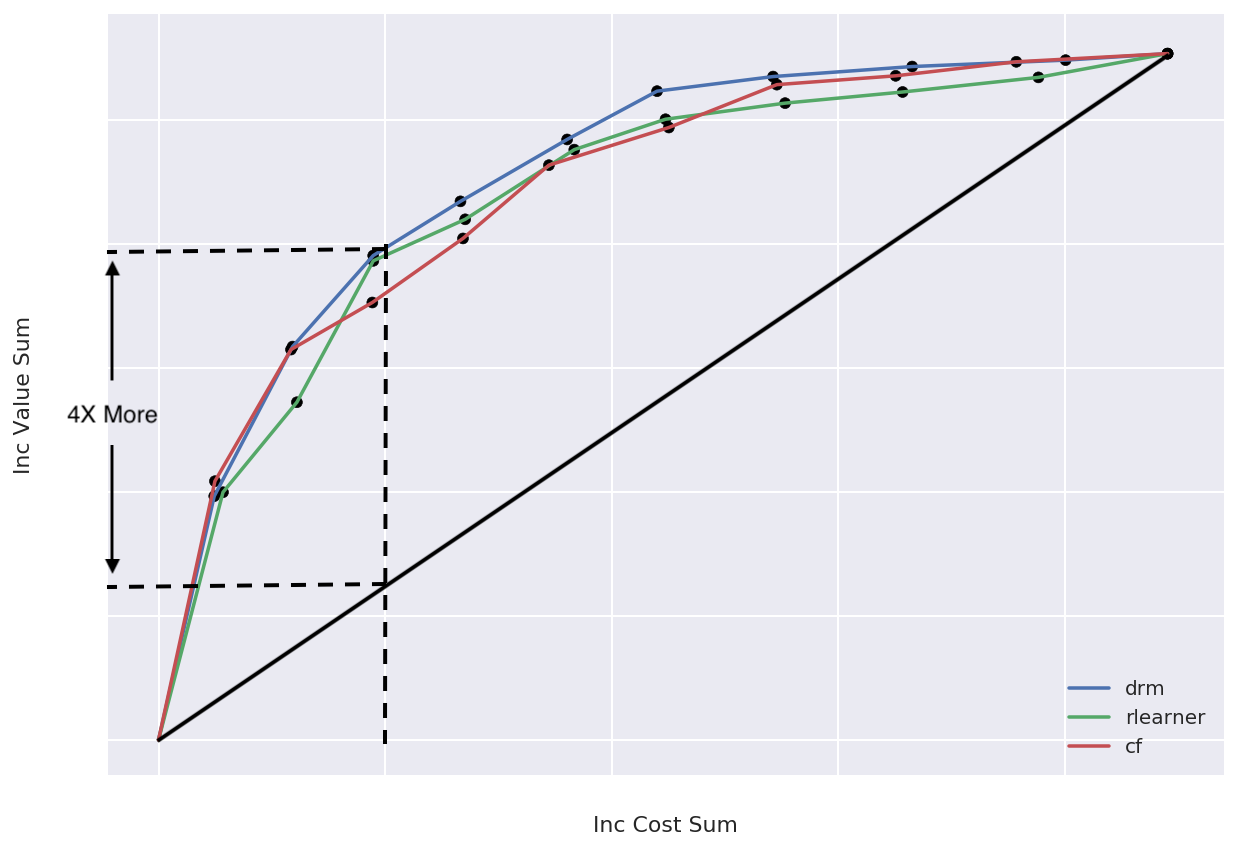
\includegraphics[height=2.2in]{cc_test_models}
\Description{Cost Curve Test}
\caption{Out-of-sample cost curve comparison for different models. DRM (blue curve) dominates other models and achieves 4X more incremental value than the benchmark given the same level of incremental cost.}
\label{fig:cc_test_models}
\end{figure}

Figure \ref{fig:cc_train_models} and second column in Table \ref{tab:2} show the performance of the models for training set. These results suggest that DRM has the most consistent performance across train and test, which demonstrate that DRM generalizes well on different data sets.

\begin{figure}
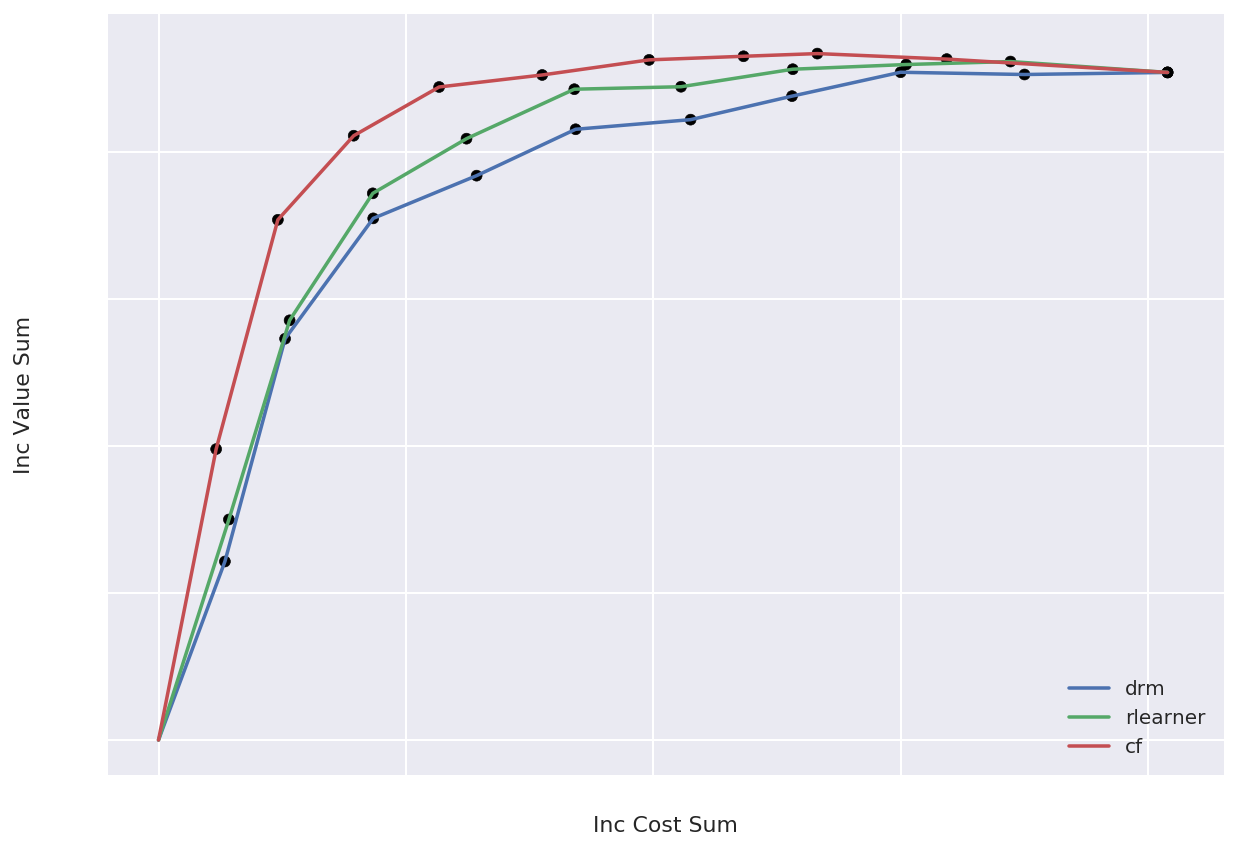
\includegraphics[height=2.2in]{cc_train_models}
\Description{Cost Curve Train}
\caption{In-sample cost curve comparison for different models. DRM (blue curve) has the worst in-sample performance but the best out-of-sample performance. This suggests DRM is more consistent and could be generalized across different data sets.}
\label{fig:cc_train_models}
\end{figure}

\subsection{Online Results}
This framework has already been deployed in production. As a multi-arm bandit \cite{kuleshov2014algorithms} case, we use an epsilon-greedy approach to keep both explore and exploit running with a certain percentage split. Both explore and exploit make promo decision based on the prediction score and corresponding threshold where explore uses a random score and exploit uses model prediction score. The threshold is determined by budget and we only send out promotions when the prediction score is above the threshold, which means we only give samples with higher score (more efficient) promotion in exploit mode.

In real-world online test, we use Eq. (\ref{eq:online_evaluation}) as the evaluation metric, which is the slope of the line between origin and one point on the cost curve.
\begin{equation}
  \label{eq:online_evaluation}
  R = \frac{ATE^r(x_i | targeted)}{ATE^c(x_i | targeted)}
\end{equation}
This measures the incremental retention per incremental cost for all samples we target in each strategy. We treat $R_{explore}$ as the benchmark and use relative performance gain Eq. (\ref{eq:relative_gain}) as the numerical metric. Note this metric is only valid when $ATE^r(x_i | targeted)$ and $ATE^c(x_i | targeted)$ are large enough and at the same scale across explore and exploit. Otherwise the efficiency ratio would not be comparable. In our online test, we monitored these values and verified that they are significantly large and at the same scale.
\begin{equation}
  \label{eq:relative_gain}
  \frac{R_{exploit}-R_{explore}}{R_{explore}}
\end{equation}

\begin{table}
  \caption{Online Treatment Efficiency Gain}
  \label{tab:3}
  \begin{tabular}{ccc}
    \toprule
    City & DRM Efficiency Gain & CF Efficiency Gain\\
    \midrule
    A & \textbf{75.3\%} & 60.2\%\\
    B & \textbf{61.5\%} & 54.3\%\\
    C & \textbf{101.2\%} & 80.4\%\\
  \bottomrule
\end{tabular}
\end{table}

Table \ref{tab:3} shows the online test results for 3 cities. They are consistent with the offline results that all models are significantly better than random explore benchmark and DRM performs better than Causal Forest in all cities. We have not included the online results for R-Learner as it is not in our production yet.


\section{Related Work}
\textbf{Promotion for user retention.} There are two recent studies by Halperin et al. \cite{halperin2018toward} and Cohen et al. \cite{cohen2018frustration}  that focus on understanding how apologies and promotions can help when the trust between user and company is compromised. In a more general study, Andrews et al. \cite{andrews2016mobile} focused on the factors that affect coupon redemption. Hanna et al. \cite{hanna2016optimizing} and Manzoor and Akoglu \cite{Manzoor2017RUSHTT} took this further and studied the redemption for time limited promotions and how different factors affect them. While these research studies use real-world data and provide insights into promotion effects, they either focus on promotion redemption or exploratory average treatment effect, which leave the headroom for heterogeneous treatment effect optimization.

\textbf{Heterogeneous Treatment Effect Estimation.} In this work, we focus on heterogeneous promotion treatment effect. The main framework for estimating treatment effect was proposed by Rubin where he studied the causal effects in randomized and non-randomized studies \cite{rubin1974estimating}. Recently, there has been a considerable interest in developing flexible and performant methods for heterogeneous treatment effect estimation. These advances include methods based on Lasso \cite{imai2013estimating}, meta learners \cite{kunzel2017meta}, recursive partitioning \cite{athey2016recursive}, causal tree and random forests \cite{wager2017estimation}, uplift tree \cite{rzepakowski2012decision}, boosting \cite{powers2017some}, neural networks \cite{louizos2017causal}, and most recently quasi-oracle estimation \cite{nie2017quasi}. A recent survey by Dorie et al. \cite{dorie2017automated} used  simulations and empirical data sets to show that these estimators can achieve good heterogeneous treatment effect estimation. However, they did not consider the special case of a constraint optimization problem where both cost and value are treatment effects.

\textbf{Optimization.} Our problem could be formed as a Knapsack problem \cite{hilliard2014algorithm}. Due to the large number of items and the small scale of the value and cost for each item, greedy approximation can achieve decent results \cite{dantzig1957discrete}. That said, this work can also use some other optimization algorithm such as SGD \cite{bottou2010large} and Adam optimizer \cite{kingma2014adam}. These two algorithms are implemented in TensorFlow \cite{abadi2016tensorflow} and provide the foundation for training of our methodology.


\section{Conclusion and Future Work}

\subsection{Conclusion}
We propose a novel ranking method to optimize heterogeneous promotion treatment effect for user retention. The method combines prediction and optimization into one single stage and provides a general loss function that can be incorporated with any differentiable functional form including linear and neural network structure. We also provide an empirical evaluation metric and adjustments for existing estimator for the promotion treatment effect optimization problem. We evaluate various methods empirically both offline and online. Our proposed method achieves significantly better performance than explore benchmark and existing estimators. After successful test, this method has been deployed to production and is live in many cities all over the world.

\subsection{Future Work}
\textbf{Sequential Learning.} In this work we only consider the treatment effect of one single promotion. But in reality, users will get promotion repeatedly and the ultimate treatment effect is the compounded effect. As a next step, we will try to estimate the sequential treatment effect and figure out the best promotion pattern for a user.

\textbf{Smart Explore/Exploit.} In current work we use epsilon-greedy explore, where we use a a fixed percentage to split the budget between exploit and a fully randomized explore. This approach is sub-optimal and sacrifices performance to blindly collect data for model training. As a better approach, we will try to use multi-arm bandit or Bayesian optimization framework to guide our smart explore based on the model uncertainty.

\textbf{Deep Embedding.} Raw time and geo features are extremely sparse. Various embedding techniques have been used for sparse features but none of them is specifically for treatment effect. As treatment effect is different from its underlying outcome, the embedding should also be different. Now that we have a general loss function which could be incorporated with any neural network structure, we could start to work on the embedding specifically for treatment effects.

%\end{document}  % This is where a 'short' article might terminate

\begin{acks}
We thank colleagues of our teams - Mo Xu, Qi Wang, Samuel Packard, Sri Kanajan, Sergey Gitlin, Charles Soll, Xuerui Wang, Kiran Vuppala, Carlos Mendoza Sanchez for useful discussion and support of this work. We thank Uber Marketplace senior scientists - Kane Sweeney, Chris Wilkins, Connan Snider and Hamid Nazer for their valuable review and feedback. We thank Prof. Stefan Wager and Xinkun Nie for their insightful discussion.

\end{acks}
